\section{Identification analysis and complements}
\subsection{Asymptotic analysis of P.E.M}
The system identification procedure:
\begin{enumerate}
\item Collect data set \textbf{u} and \textbf{y}
\item Select class of parametric models $m(\theta)$
\item Find the best in-class model $m(\hat{\theta}) : \hat{\theta}=argmin_{\theta}\{J_N({\theta}\})$
\end{enumerate}
Is the model $m(\hat{\theta})$ a \textbf{good} model?\\
To make a clean theoretical analysis we move into asymptotic quantities :
$$ J_N(\theta)=\frac{1}{N}\sum\limits_{t=1}^{N}\epsilon(t,\theta)^2 \xrightarrow[]{N \to \infty} \bar{J}(\theta)=E[\epsilon(t,\theta)^2]$$
$J_N(\theta)$ is the \textbf{real} performance index which makes an average over \textbf{time}. $\bar{J}(\theta)$ is the \textbf{asymptotic} performance index which makes an average over \textbf{events}.\\
We can assume that $J_N(\theta) \to \bar{J}(\theta)$ if $\epsilon(t,\theta)$ is an \textbf{ergodic process} , a process where we can compute expected values over events  using expected values over time.\\
Consider $\bar{J}(\theta)$ and assume that it has a unique global minimum :
$$ \bar{\theta} : \bar{J}(\theta) \geq \bar{J}(\bar{\theta}) \forall \theta \in \Re^{n_{\theta}}$$
If $J_N(\theta) \to \bar{J}(\theta)$ we can assume that $ \hat{\theta}_N \to \bar{\theta}$
Now lets assume that the \textbf{real system S} that has generated the dataset is within the model class : $ \text{\textbf{S}} \in m(\theta) \to a\theta ^0$  exists so that $ m(\theta^0) = \text{\textbf{S}}$.
$$ \text{Is } \theta^0 = \bar{\theta} \text{?}$$
In other words , is the P.E.M performance index able to select the \textbf{true} parameter $\theta^0$.
\begin{description}
\item[Proof]\hfill\\
Consider the prediction error $\epsilon(t,\theta) = y(t) - \hat{y}(t|t-1,\theta)$.
Add on both sides $ -\hat{y}(t|t-1,\theta^0)$:
$$ \epsilon(t,\theta) -\hat{y}(t|t-1,\theta^0) = y(t) - \hat{y}(t|t-1,\theta) -\hat{y}(t|t-1,\theta^0)$$
Where $y(t)-\hat{y}(t|t-1,\theta^0)$ is the \textbf{white noise} e(t) of the true system \textbf{S}.
$$ \epsilon(t,\theta)=e(t)-(\hat{y}(t|t-1,\theta^0)-\hat{y}(t|t-1,\theta))$$
Square and apply expected value:
$$ E[\epsilon(t,\theta)^2]=E[e(t)^2]+E[(\hat{y}(t|t-1,\theta^0)-\hat{y}(t|t-1,\theta))^2]+2E[e(t)(\hat{y}(t|t-1,\theta^0)-\hat{y}(t|t-1,\theta))]$$
The last term is =0 because e(t) cannot be correlated with $\hat{y}(t|t-1,\theta)$ or $\hat{y}(t|t-1,\theta^0)$. Remembering that $E[\epsilon(t,\theta)^2]= \bar{J}(\theta)$ and $E[e(t)^2]=var[e(t)] = \lambda^2$ :
$$ \bar{J}(\theta) = \lambda^2 + E[(\hat{y}(t|t-1,\theta^0)-\hat{y}(t|t-1,\theta))^2]$$
\[  E[(\hat{y}(t|t-1,\theta^0)-\hat{y}(t|t-1,\theta))^2]=
  \begin{cases}
    \geq 0       & \quad \text{if } \theta \neq \theta^0\\
   	 0  			 & \quad \text{if } \theta = \theta^0
  \end{cases}
\]
So $\bar{J}(\theta) \geq \lambda^2 = \bar{J}(\theta^0)$ which means that $\theta^0$ is the global minimum of $\bar{J}(\theta) $ $$ \bar{\theta} = \theta^0$$ The P.E.M provides the \textbf{true model} if \textbf{S} $\in m(\theta)$ 
\item[Remark 1]\hfill\\
If \textbf{S} $\in m(\theta)$ then $\epsilon(t,\theta^0) \approx \epsilon(t,\hat{\theta}_N)=$WN.\\
We can use this result to check (\textbf{a-posteriori}) if the estimated model $m(\hat{\theta}_N)$ is the true model by performing a \textbf{whiteness test} on the signal:
$$ \epsilon(t,\hat{\theta}), t=1,2,...,N$$
This is a practical way to make a final \textbf{validation} of the identification procedure.
\newpage
\item[Remark 2]\hfill\\
\begin{enumerate}
\item \textbf{S} $\in m(\theta) \to \bar{\theta} = \theta^0$
\begin{figure}[H]
 \centering
  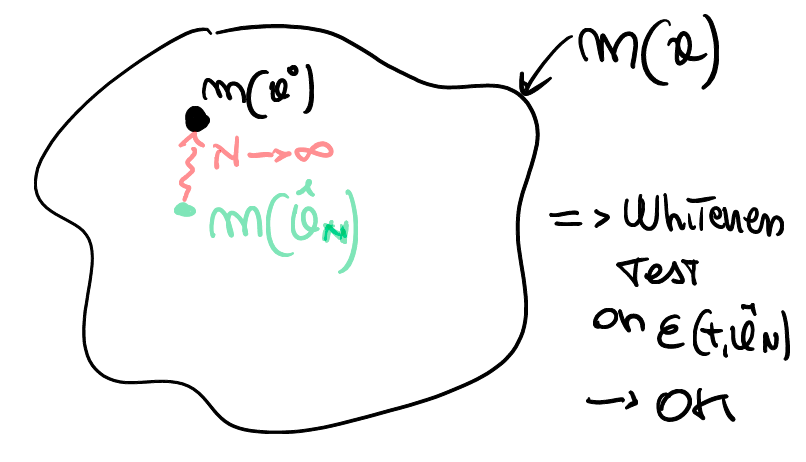
\includegraphics[width=.5\linewidth]{whiteness_test1}
\end{figure}
\item \textbf{S} $\notin m(\theta) \to \bar{\theta} \neq \theta^0  $
\begin{figure}[H]
 \centering
  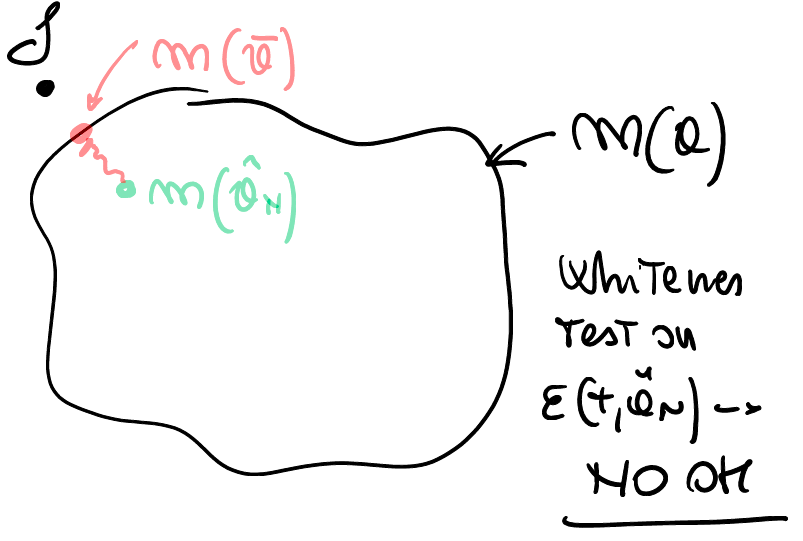
\includegraphics[width=.5\linewidth]{whiteness_test2}
\end{figure}
Best you can do is get as close as possible to S within model class $m(\theta)$
\end{enumerate} 
\end{description}

\subsection{Model-order selection}
In the system identification procedure we make 2 critical choices : 
\begin{enumerate}
\item ARMA or ARMAX ?
\item Model order ? (ARMA(m,n)/ARMAX(m,n,p))
\end{enumerate}
For ARMA the total order is $n= m+n$ and represents a \textbf{2-D} order problem, while for ARMAX the total order is $n=m+n+p$ and represents a \textbf{3-D} order problem.\\
To simplify the problem to a \textbf{1-D} problem we make the assumption of using \textbf{balanced models} ($m \approx n \approx p$).\\
What is the best \textbf{global} order of $n_{\theta}$?\\
Intuitively ,select $n_{\theta} \to \text{find  } \hat{\theta}_N \text{; compute  } J_N(\hat{\theta}_N; n_{\theta})$ (use the $n_{\theta}$ that provides the minimum $J_N(\hat{\theta}_N)$
which is a \textbf{totally wrong} approach because:
$$ J_N(\hat{\theta}_N) \xrightarrow[]{n_{\theta} \to \infty} 0$$
Even stricter:
$$ J_N(\hat{\theta}_N) \xrightarrow[]{n_{\theta} \to N} 0$$
So if the number of parameters is equal to the number of data we obtain error = 0, which is bad because we will never achieve \textbf{generalisation}.
There are 3 main approaches to find the best $n_{\theta}$ under the following assumptions:
\begin{itemize}
\item A batch of N measured data is available
\item We test increasingly model orders $n_{\theta}=1,2,3...$
\item $J_N(\hat{\theta}_N;n_{\theta})$ is the performance index computed on its best parameter vector which is dependent on $n_{\theta}$.
\end{itemize}

\subsubsection{Discontinuity search}
Algorithm :
\begin{itemize}
\item Select a value of $n_{\theta}$
\item Find $\hat{\theta}_N$
\item Compute $J_N(\hat{\theta}_N)$
\item Make \textbf{whiteness test} on $\epsilon(t,\hat{\theta}_N)=y(t)-\hat{y}(t|t-1;\hat{\theta}_N)$
\item Repeat procedure for $n_{\theta}=1,2,3...$
\end{itemize}
Ideally , by plotting the graph of performance index and model-order a \textbf{discontinuity} should be visible. The \textbf{optimal} value for $n_{\theta}$ is the smallest after said discontinuity.
\begin{figure}[H]
 \centering
  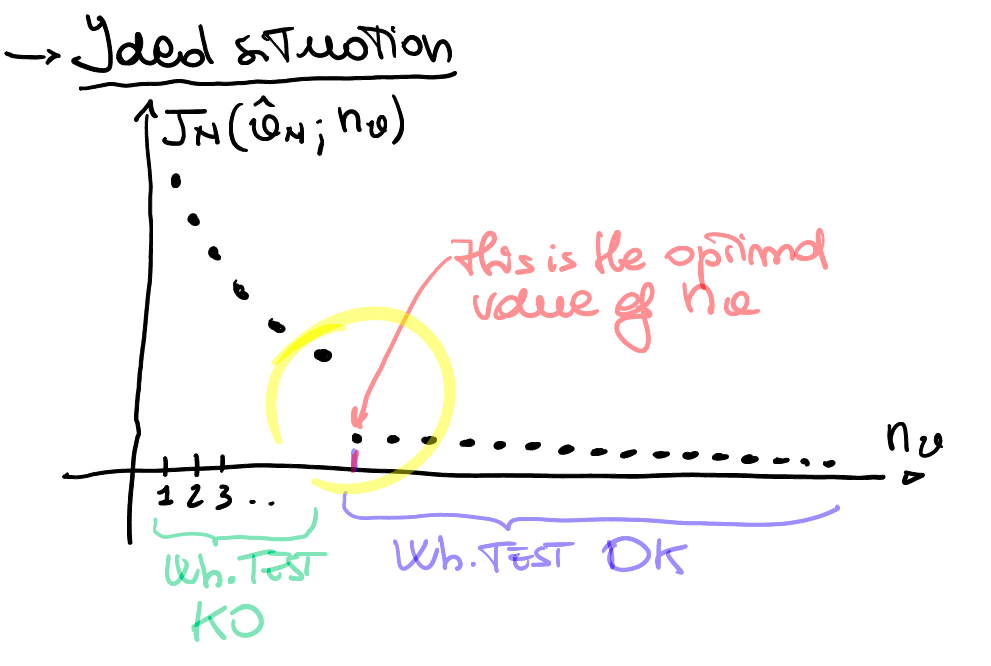
\includegraphics[width=.5\linewidth]{discont_id}
\end{figure}
What happens \textbf{really} is that there is no real discontinuity rather than a \textbf{region of values} which hold the optimal solution.In that region the whiteness test is still passed but with \textbf{low confidence} levels.
\begin{figure}[H]
 \centering
  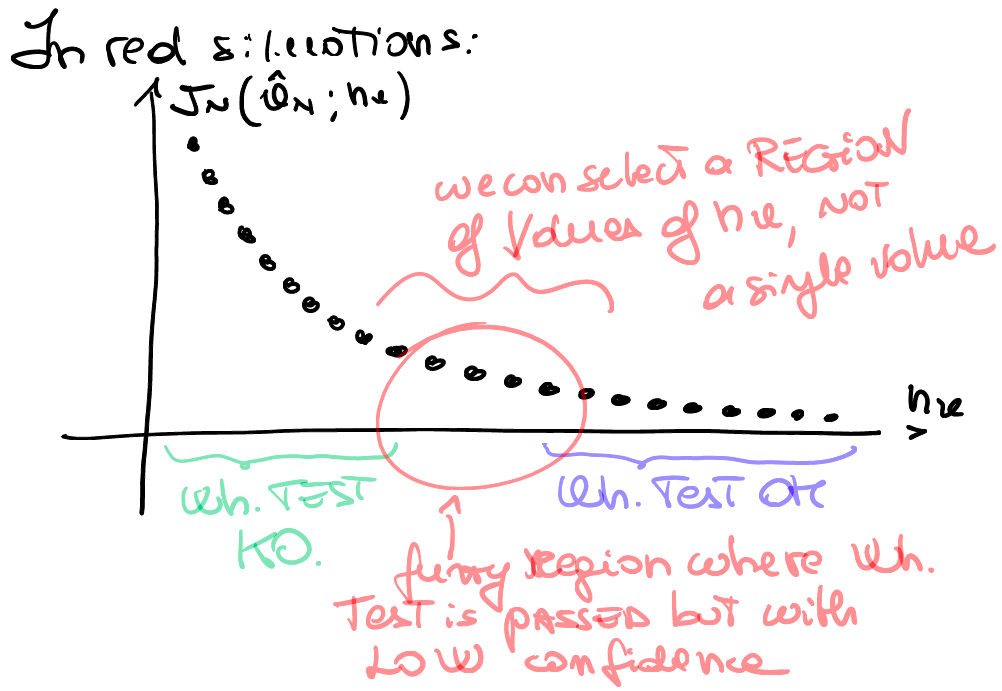
\includegraphics[width=.5\linewidth]{discont_re}
\end{figure}

\subsubsection{Cross validation}
Suppose we have a set of N dataset points. We divide this data set in two subsets
\begin{itemize}
\item \textbf{Identification/Learning} dataset\\
$\Phi_i =1 \to \frac{N}{2}$
\item \textbf{Validation} dataset\\
$\Phi_v =1 \frac{N}{2}+1 \to N$
\end{itemize}
Procedure :
\begin{enumerate}
\item Define a model order $n_{\theta}$
\item Find $\hat{\theta}_{\frac{N}{2}}$ by minimizing $J_{\frac{N}{2}}(\theta;\Phi_i;n_{\theta})$
\item Compute  $J_{\frac{N}{2}}(\hat{\theta}_{\frac{N}{2}};\Phi_i;n_{\theta})$ and $J_{\frac{N}{2}}(\hat{\theta}_{\frac{N}{2}};\Phi_v;n_{\theta})$ 
\item Repeat for $n_{\theta}=1,2,3...$
\end{enumerate}
\begin{figure}[H]
 \centering
  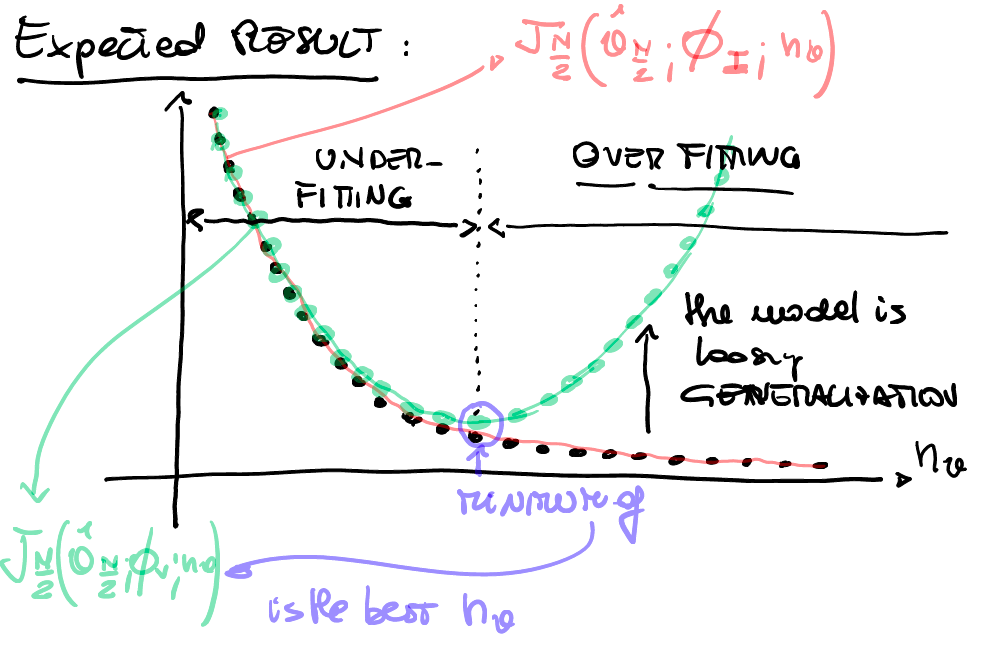
\includegraphics[width=.5\linewidth]{cross_val}
\end{figure}
In the over-fitting region the estimated model fits \textbf{not only} the specific dynamics of the system but also the \textbf{noise} which results in loosing \textbf{generality}.\\
\begin{description}
\item[Drawbacks of crossvalidation]\hfill\\
We are forced to used just $\frac{N}{2}$ data points instead of N data points.
This is not an issue for N large ($\sim 100.000$) but is an issue for N small ($\sim 500$)
\end{description}


\subsubsection{Estimation criteria}
\begin{enumerate}
\item \textbf{Find prediction error (FPE)}\\
\[
\boxed{\text{FPE}(n_{\theta})= \frac{N+n_{\theta}}{N-n_{\theta}} J_N(\hat{\theta}_N,n_{\theta})}
\]
The first part $\frac{N+n_{\theta}}{N-n_{\theta}}$ is an \textbf{increasing function } while the second part $J_N(\hat{\theta}_N,n_{\theta})$ is a \textbf{decreasing} function.\\
The FPE is a modification of the original performance index and has a \textbf{minimum}.
\begin{figure}[H]
 \centering
  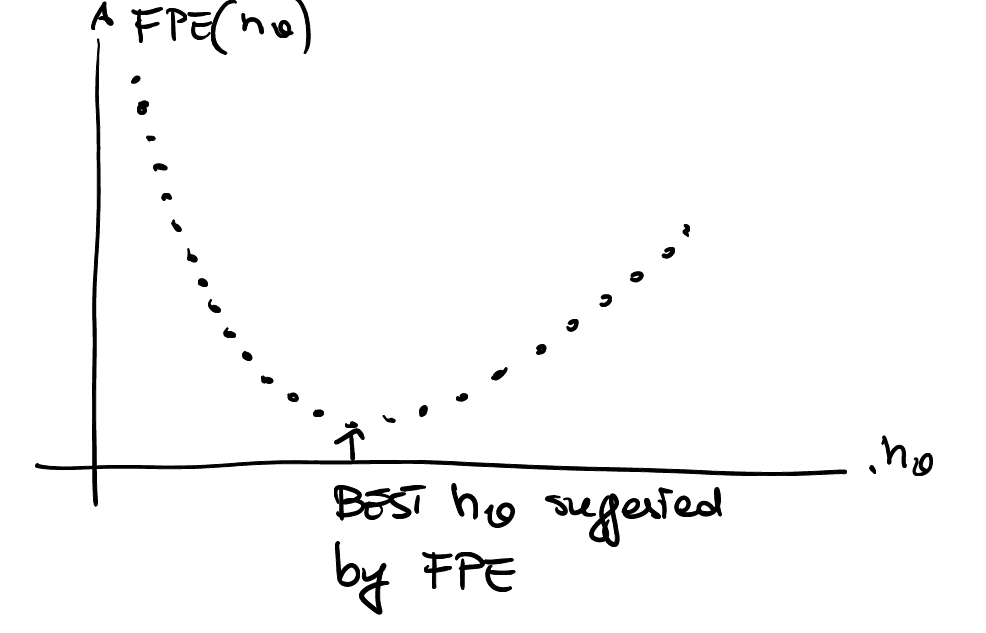
\includegraphics[width=.4\linewidth]{FPE}
\end{figure}
\item \textbf{Akaike Information Criterion (AIC)}\\
\[
\boxed{AIC(n_\theta) = 2 \frac{n_{\theta}}{N}+ ln(J_N(\hat{\theta},n_{\theta}))}
\]
Again the first part is increasing while the second is decreasing.
\item \textbf{Minimum description length (MDL)}\\
\[
\boxed{MDL(n_{\theta}=ln(N)\frac{n_{\theta}}{N}+ln(J_N(\hat{\theta},n_{\theta}))}
\]
Again the first part is increasing while the second is decreasing.
\end{enumerate}
\begin{figure}[H]
 \centering
  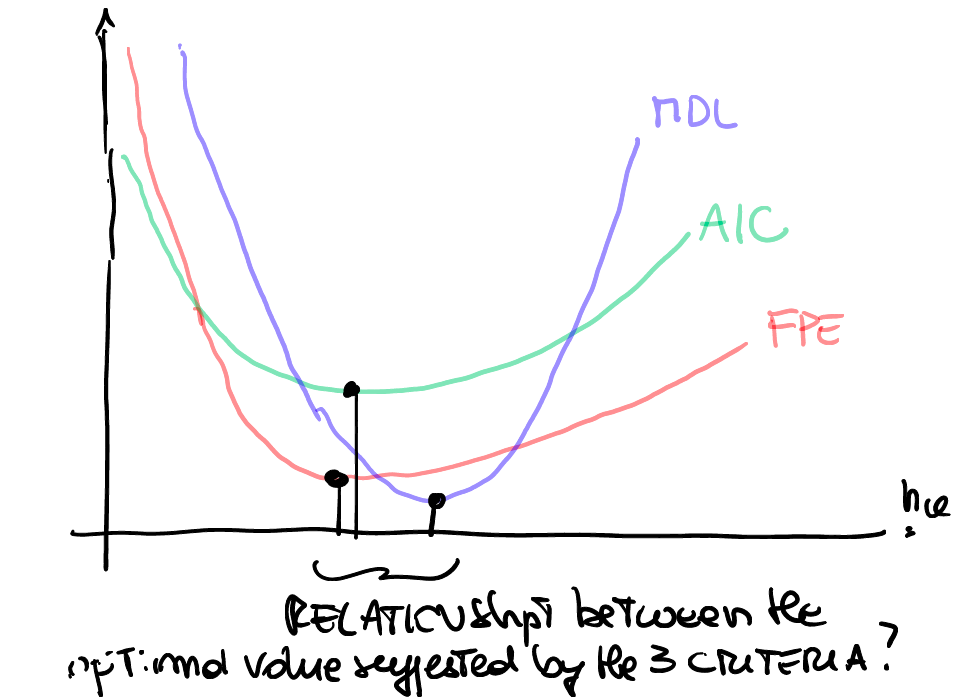
\includegraphics[width=.5\linewidth]{criteria_comparison}
\end{figure}


\subsubsection{Comparison between FPE and AIC}
$$ ln(FPE) = ln(\frac{N+n_{\theta}}{N-n_{\theta}} J_N(\hat{\theta}_N,n_{\theta}))$$
$$ ln(FPE) = ln(\frac{1+\frac{n_{\theta}}{N}}{1-\frac{n_{\theta}}{N}} J_N(\hat{\theta}_N,n_{\theta}))$$
\newpage
\par\noindent\rule{\textwidth}{0.4pt}

\begin{description}
\item[Remark]\hfill\\
Remind that $ln(1+x) \approx x \text{ when } x=0$
\end{description}
\par\noindent\rule{\textwidth}{0.4pt}
\\If $n_{\theta}<<N \to \frac{n_{\theta}}{N} \approx 0$ so :
$$ ln(1+\frac{n_{\theta}}{N}) - ln(1-\frac{n_{\theta}}{N}) + ln(J_N(\hat{\theta};n_{\theta})) \approx \frac{n_{\theta}}{N}-(-\frac{n_{\theta}}{N})+ln(J_N(\hat{\theta};n_{\theta}))$$
$$ 2\frac{n_{\theta}}{N}+ln(J_N(\hat{\theta};n_{\theta})) = AIC(n_{\theta})$$
So if $n<<N$ (always true in predicted applications):
\[
\boxed{ln(FPE) = AIC	}
\]
Notice that if f(x) has a minimum in $x_0$ then also $ln(f(x))$ has a minimum in $x_0 \to \frac{d}{dx}(ln(f(x))) = \frac{1}{f(x)}f'(x)$ :
\[
\boxed{argmin_{\theta}\{FPE(n_{\theta}\}=argmin_{\theta}\{AIC(n_{\theta}\}}
\] 
So FPE and AIC provide the \textbf{same optimal} value for $n_{\theta}$

\subsubsection{Comparison between AIC and MDL}
$$ AIC(n_\theta) = 2 \frac{n_{\theta}}{N}+ ln(J_N(\hat{\theta},n_{\theta})) $$
$$ MDL(n_{\theta}=ln(N)\frac{n_{\theta}}{N}+ln(J_N(\hat{\theta},n_{\theta}))$$
Only difference in is $2 \frac{n_{\theta}}{N} \text{ vs } ln(N)\frac{n_{\theta}}{N} $
AIC and MDL provide \textbf{slightly } different results , if $ln(N) > 2$ AICF(FPE) suggest a \textbf{bigger} solution than MDL.\\
\begin{itemize}
\item \textbf{AR/ARX}\\
If \textbf{S} the real system is an AR/ARX system , \textbf{MDL} is theoretically the correct indication of \textbf{best value}
\item \textbf{ARMA/ARMAX}\\
If \textbf{S} is an ARMA/ARMAX , \textbf{AIC(FPE)} should be used.
\end{itemize}
\newpage
\subsection{Design of experiment}
Given data sets \textbf{u} and \textbf{y} and considering a generic \textbf{ARX(m,p+1)} model class we can use the P.E.M approach to solve the identification problem using Least Squares :
$$ \hat{\theta}_N = (\sum\limits_{t=1}^{N} \phi(t)\phi^T(t))^{-1}(\sum\limits_{t=1}^{N}y(t)\phi(t))$$ 
We have a unique solution if $(\sum\limits_{t=1}^{N} \phi(t)\phi^T(t))^{-1}$ is \textbf{ invertible}. When is it invertible?\\
Focusing on condition $u(t)$, we can in some situations \textbf{design} the input signal \textbf{u}$=\{u(1),...,u(N)\}$.Define:
$$ S(N) = \sum\limits_{t=1}^{N} \phi(t)\phi^T(t) $$
$$ R(N) = \frac{1}{N}S(N)$$
So :
$$ \hat{\theta}_N = R(N)^{-1}(\sum\limits_{t=1}^{N}y(t)\phi(t))$$ 
We will focus on the \textbf{asymptotic} value of $R(N) \xrightarrow[]{N \to \infty}  \bar{R}$ . The problem is now : when is $\bar{R}$ \textbf{invertible}?\\
In a generic ARX(m,p+1) $\bar{R}$ has the following structure:
$$ \bar{R}= 
\begin{array}{c|c}
  \bar{R}_y & -\bar{R}_{y\mu} \\ 
  \hline
  -\bar{R}_{\mu y} & \bar{R}_{\mu}
 \end{array}$$

\begin{itemize}
\item $\bar{R}_y$\\
Is an m x m \textbf{covariance} matrix of order m-1 of the signal y(t):

$$
\bar{R}_y = 
	\begin{bmatrix}
       \gamma_{y}(0) & \gamma_y(1) & ... & \gamma_y(m-1)        \\[0.3em]
       \gamma_y(1) & \gamma_y(0)\gamma_y(1) &...& \gamma_y(m-2) \\[0.3em]
       ... & ... & ... 	& ...								   \\[0.3em]
       \gamma_y(m-1) & ... & ... & \gamma_y(0)
     \end{bmatrix} 
$$

\item $\bar{R}_{u}$\\
Is a $(p+1)$ x $(p+1)$ \textbf{covariance } matrix of order p of signal u(t):
$$
\bar{R}_{u} = 
	\begin{bmatrix}
       \gamma_{u}(0) & \gamma_{u}(1) & ... & \gamma_{u}(p)        \\[0.3em]
       \gamma_{u}(1) & \gamma_{u}(0)\gamma_{u}(1) &...& \gamma_{u}(p-1) \\[0.3em]
       ... & ... & ... 	& ...								   \\[0.3em]
       \gamma_{u}(p) & ... & ... & \gamma_{u}(0)
     \end{bmatrix} 
$$

\item $\bar{R}_{yu}$\\
Is a m x $(p+1)$ \textbf{cross-variance} matrix between y(t) and u(t):
$$
\bar{R}_{yu} = 
	\begin{bmatrix}
       \gamma_{yu}(0) & \gamma_{yu}(1) & ... & \gamma_{yu}(p)        \\[0.3em]
       \gamma_{yu}(1) & \gamma_{yu}(0)\gamma_{yu}(1) &...& \gamma_{yu}(p-1) \\[0.3em]
       ... & ... & ... 	& ...								   \\[0.3em]
       \gamma_{yu}(m-1) & ... & ... & \gamma_{yu}(0)
     \end{bmatrix} 
$$
\item $\bar{R}_{u y}$\\
Is $\bar{R}_{u y} = \bar{R}_{yu}^T$
\end{itemize}
\par\noindent\rule{\textwidth}{0.4pt}
\begin{description}
\item[Remark : Lemma di Schur]\hfill\\
Given a \textbf{block matrix}  
$$ M= 
\begin{array}{c|c}
  F & K \\ 
  \hline
  K^T & H
 \end{array}$$
 where F,H are \textbf{square} and \textbf{symmetric} matrices then $M>0$ if and only if:
\begin{itemize}
\item $ \text{\textbf{H}} > \text{\textbf{0}}$
\item $\text{\textbf{F-KH}}^{-1}\text{\textbf{K}}^T > 0$
\end{itemize}
\end{description}
\par\noindent\rule{\textwidth}{0.4pt}
\\The important part from Schur's Lemma is that $H>0$ which refers to the part of $\bar{R}_{u}$ containing only u(t).
The condition that must hold for $\bar{R}$ to be \textbf{invertible} is
\[
\boxed{\bar{R}_u >0}
\]

Let's define the covariance matrix of $u(t)$ of order i (i x i matrix) :
$$
\bar{R}^{(i)}_{u} = 
	\begin{bmatrix}
       \gamma_{u}(0) & \gamma_{u}(1) & ... & \gamma_{u}(i-1)            \\[0.3em]
       \gamma_{u}(1) & \gamma_{u}(0) &...  & \gamma_{u}(i-2)          \\[0.3em]
       ... & ... & ... 	& ...								   \\[0.3em]
       \gamma_{u}(i-1) & ... & ... & \gamma_{u}(0)
     \end{bmatrix} 
$$

A signal $u(t)$ is \textbf{persistently exciting} of order n if:
\[
\boxed{ \bar{R}^{(1)}_{u} >0, \bar{R}^{(2)}_{u} >0 ,...,\bar{R}^{(n)}_{u} > 0 , \bar{R}^{(n+1)}_{u} \geq 0,... }
\]
The maximum order is n so , n is the order of $\bar{R}^{(i)}_{u}$ such that this matrix is \textbf{invertible}.\\ In Conclusion:\\ \hspace{1cm}

\fbox{\begin{minipage}{30em}
\centering
A necessary condition for the identification process of an ARX(m,p+1) model is that the input signal u(t) must be \textbf{persistently exciting} of order at least \textbf{p+1}
\end{minipage}}
\\

\par\noindent\rule{\textwidth}{0.4pt}
\begin{description}
\item[Remark 1: WN]\hfill\\
Notice that if $u(t) \approx WN(0,\lambda^2)$ :
$$
\bar{R}^{(i)}_{u} = 
	\begin{bmatrix}
        \lambda^2 & 0 & ... & 0           \\[0.3em]
       0 & \lambda^2 &...  & 0          \\[0.3em]
       ... & ... & ... 	& ...								   \\[0.3em]
       0 & ... & ... & \lambda^2
     \end{bmatrix} = \lambda^2 I^{(i)}
$$
A WN is \textbf{persistently exciting} signal of order $\infty$
\item [Remark 2: Sinusoid]\hfill\\
$u(t) =Asen(wt)$  is a \textbf{persistently exciting signal} of order \textbf{2}.
If possible the best choice for $u(t)$ is a WN!
\newpage
\item [Remark 3 : Practical application WN or BLWN?]\hfill\\
\begin{figure}[H]
 \centering
  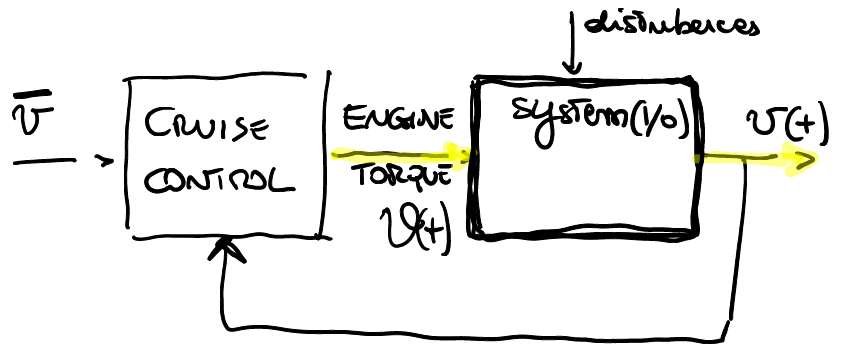
\includegraphics[width=.6\linewidth]{cruise_control}
\end{figure}
Problem : design a block box model of the system, starting from an \textbf{excitation} experiment.How to design the experiment?\\
\begin{figure}[H]
 \centering
  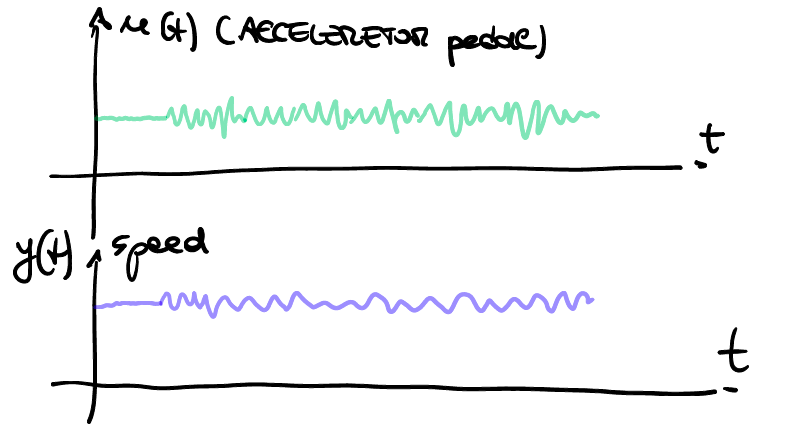
\includegraphics[width=.5\linewidth]{signals}
\end{figure}
In principle $u(t)$ corresponding to the input of the acceleration pedal can be modelled as a WN ( allows complete excitation). This is \textbf{not} a good solution though because a lot of excitation energy is used on a \textbf{useless} bandwidth.
Assuming that the bandwidth of the cruise control system is about 2Hz  using the \textbf{full-bandwidth} up to $w = \pi $ is \textbf{useless}. A better choice would be a \textbf{band limited white noise (BLWN)} which focuses its attention of the system identification procedure on the \textbf{relevant frequency range} $[0 , \text{just beyond control bandwith}]$.
\end{description}
\par\noindent\rule{\textwidth}{0.4pt}

\subsection{Uncertainty evaluation of a parametric identification algorithm}
Assume that \textbf{S} $\in m(\theta)$ then there exists a single parameter vector which represents the \textbf{true} system:$$ \theta^0 = \bar{\theta}$$
In practice we can only use a \textbf{finite number} of data points (\textbf{N}) which means that $\hat{\theta}_N$ depends on N.Notice that $\hat{\theta}_N$ is also a vector of  \textbf{random variables} such that $$ E[\hat{\theta}_N]=\theta^0$$
But is it also true that $$ var[\hat{\theta}_N]=?=E[(\hat{\theta}_N - \theta^0)(\hat{\theta}_N - \theta^0)^T]$$
The covariance matrix of $\hat{\theta}_N$ provides an estimation of the \textbf{uncertainty}  in the estimation of $\theta^0$ using $\hat{\theta}_N$.\\
It can be proven that :
\[
\boxed{var[\hat{\theta}_N] = \frac{1}{N}\lambda^2 \bar{C}^{-1}}
\]
where 
$$ \lambda^2 = var[e(t)]=var[y(t) - \hat{y}(t|t-1,\theta^0)]$$
$$ \bar{C}= E\left[ \left. \frac{\partial{\epsilon(t,\theta)}}{\partial{\theta}}\right|_{\theta=\theta^0} \cdot \left. \frac{\partial{\epsilon(t,\theta)}}{\partial{\theta}}\right|^{T}_{\theta=\theta^0} \right]$$
Practical computation of $var[\hat{\theta}_N]$:
$$ \lambda^2 = E[e(t)^2] \approx \frac{1}{N} \sum\limits_{t=1}^{N}(y(t) - \hat{y}(t|t-1,\hat{\theta}_N)$$

$$\bar{C} \approx \frac{1}{N}\sum\limits_{t=1}^{N}\left( \left. \frac{\partial{\epsilon(t,\theta)}}{\partial{\theta}}\right|_{\theta=\hat{\theta}_N} \cdot \left. \frac{\partial{\epsilon(t,\theta)}}{\partial{\theta}}\right|^{T}_{\theta=\hat{\theta}_N} \right)$$

First approximation : instead  of using expected value $\to$ average over \textbf{time}.\\
Second approximation : instead of using $\theta^0 \to \hat{\theta}_N$

\subsubsection{Interpretation of $\bar{C}$}
$$\bar{J}(\theta) = E[\epsilon(t,\theta)^2]$$
$$ \frac{\partial{\bar{J}(\theta}}{\partial{\theta}}=E \left[ 2\epsilon(t,\theta)\frac{\partial{\epsilon(t,\theta)})}{\partial{\theta}}\right] $$
$$ \frac{\partial^2{\bar{J}(\theta)}}{\partial{\theta^2}}=E \left[ 2\frac{\partial{\epsilon(t,\theta)}}{\partial{\theta}}\frac{\partial{\epsilon(t,\theta)}}{\partial{\theta}}^T + 2\epsilon(t,\theta)\frac{\partial^2{\epsilon(t,\theta)}}{\partial{\theta^2}}\right] $$
If $\hat{\theta}_N = \theta ^0 \to \epsilon(t,\theta) = e(t)$ :
$$ \left. \frac{\partial^2{\bar{J}(\theta)}}{\partial{\theta^2}} \right|_{\theta=\theta^0}=E \left[ \left. 2\frac{\partial{\epsilon(t,\theta)}}{\partial{\theta}}\right|_{\theta=\theta^0} \left. \frac{\partial{\epsilon(t,\theta)}}{\partial{\theta}}\right|^{T}_{\theta=\theta^0} + \left. 2e(t)\frac{\partial^2{\epsilon(t,\theta)}}{\partial{\theta^2}}\right|_{\theta=\theta^0} \right] $$
Due to \textbf{non} correlation :
$$ \left. \frac{\partial^2{\bar{J}(\theta)}}{\partial{\theta^2}} \right|_{\theta=\theta^0}=E \left[ \left. 2\frac{\partial{\epsilon(t,\theta)}}{\partial{\theta}}\right|_{\theta=\theta^0} \left. \frac{\partial{\epsilon(t,\theta)}}{\partial{\theta}}\right|^{T}_{\theta=\theta^0} \right] =2\bar{C} $$
\[
\boxed{\bar{C} = \frac{1}{2}\left. \frac{\partial^2{\bar{J}(\theta)}}{\partial{\theta^2}} \right|_{\theta=\theta^0}}
\]
\begin{itemize}
\item The estimation error has a \textbf{larger} variance for \textbf{larger} values of $\lambda^2$ (size of of the WN at the input of the system)
\item The estimation error has a \textbf{larger} variance for \textbf{smaller} values of N.
\item The estimation error  has a \textbf{larger } variance if the \textbf{second derivative} of the performance index around the global minimum $\theta^0$ is \textbf{smaller}
\begin{figure}[!h]
\begin{minipage}{.5\textwidth}
 \centering
  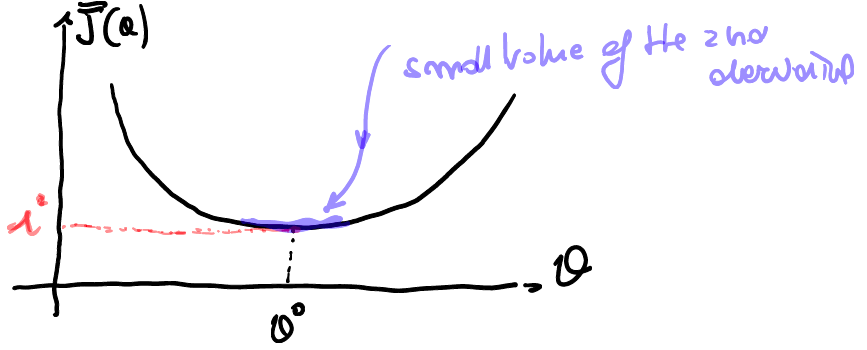
\includegraphics[width=.8\linewidth]{small_hessian}
\end{minipage}%
	\begin{minipage}{.5\textwidth}
  \centering
  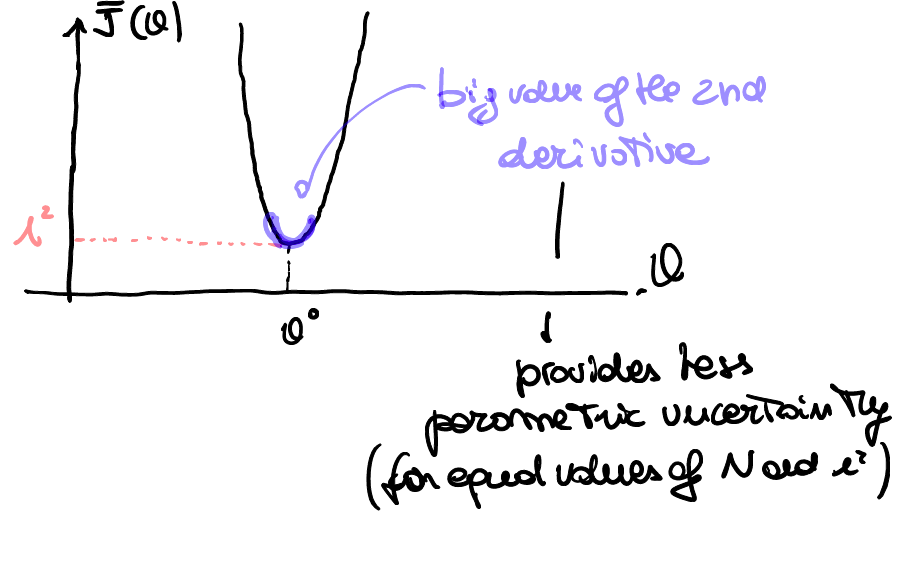
\includegraphics[width=.8\linewidth]{big_hessian}
\end{minipage}%
\end{figure}
\end{itemize}
With this formula we can understand if the number of data is \textbf{enough} to provide the requested level of uncertainty in parameter estimation.